\documentclass[a4paper]{article}
% Eso define el tipo de documento.
% `article` se divide en secciones y tiene el resumen pegado al texto
\usepackage{graphicx}
% Son como los import de librerias. `graphicx` es para importar imagenes
\usepackage{listings}
% `listings` es para insertar los codigo fuente
\usepackage[utf8]{inputenc}
% `utf8` es para no tener problemas con el encoding (acentos, etc.)
\usepackage{caption}
% Para cambiar leyenda de figuras

\title{Trabajo Práctico Nro. 2:\\“Puertos Analógicos”}
\author{Amodey, Leandro - leandroamodey@gmail.com
\and Monti, Matías - matiasmonti@hotmail.com
\and Quinteros, Fernando - lordfers@gmail.com
\and Araneda, Alejandro – eloscurodeefeso@hotmail.com}
\date{1er. Cuatrimestre 2020\\Lunes, 11 de Mayo, 8hs.}
% `title`, `author` y `date` es informacion que todos los archivos tienen.

\def\teacher{Ing. Jorge H. Doorn
\and Ing. Matías Presso}
% Variable propia para definir profesores.

\captionsetup{labelsep=period,font={small},labelfont=bf,textfont=it}
% Las leyendas deben ser chicas y en italica, separadas con punto
% y la numeración en negritas 
\renewcommand{\figurename}{Figura}
% Con eso cambiamos como salen los titulos de las figuras.
\renewcommand{\abstractname}{Resumen}
% Con eso le cambio en titulo del resumen
\renewcommand{\refname}{Referencias}
% Cambia el titulo de la bibliografia
\let\originalcite\cite
\renewcommand{\cite}[2][]{\textsuperscript{\originalcite{#2}}}
% Cambiamos el estilo de las citas bibliograficas
\makeatletter\let\@afterindentfalse\@afterindenttrue\makeatother
% Cambiamos \@afterindentfalse por \@afterindenttrue para indentar primer parrafo
\let\originalappendix\appendix
\renewcommand{\appendix}{%
    \newpage\originalappendix\pagenumbering{gobble}%
    % Empezar apéndices en nueva pagina sin numeracion
    \renewcommand\thesection{Anexo \Alph{section}}
    % `thesection` es como se numeran los apendices
    \setcounter{secnumdepth}{1}
    % Contarlas secciones de apendice
}
\setcounter{secnumdepth}{0}
% No se numeran las secciones pero si estan en el TOC 
\newenvironment{ejercicios}
    {\setcounter{secnumdepth}{3}
    \renewcommand\thesubsection{Ejercicio \arabic{subsection}}}
    {\setcounter{secnumdepth}{0}}
% Defino un enviroment para numerar ejercicios

% Defino un enviroment para numerar Conceptos:
\newenvironment{Conceptos}
    {\setcounter{secnumdepth}{1}
    \renewcommand\thesubsection{Concepto \arabic{subsection}}}
    {\setcounter{secnumdepth}{0}}

\begin{document}
% Arranca el documento

% Pagina propia de titulo
\begin{titlepage}\renewcommand\and\par\centering\makeatletter
    
\includegraphics{logo.png}\par
    {\Large Ingeniería en Computación \par}\vspace{0.5cm}
    {\LARGE Laboratorio de Microprocesadores \par}\vfill
    {\huge \@title \par}\vfill
    Grupo 2:\par
    \@author\vfill
    Práctica entregada:\par
    \@date\vfill
    Docentes:\par
    \teacher\vspace{1cm}\makeatother
\end{titlepage}

\begin{abstract}

    En el presente trabajo ejemplificaremos mediante diversar 
    aplicaciones la utilización de los módulos analógicos de un 
    microcontrolador. A su vez, éstas ilustrarán la forma en que el 
    diseño digital que en general pertenece al dominio de la 
    corriente contínua y de baja tensión, se relaciona con los 
    componentes electrónicos propios también de la corriente alterna 
    y de mayor tensión.

\end{abstract}

\section{Introducción}

\subsection*{Características de las entradas A/D}
    
\subsubsection*{Comparador Analógico}
	El PIC12F675 tiene un comparador analógico, y las entradas al
	comparador se multiplexan con los pines GP0 y GP1.
	Además, GP2 se puede configurar como salida del comparador.
	El registro de control del comparador (CMCON) contiene
	los bits para controlarlo.
	
	En la Figura 3 se muestra un solo comparador, junto con
	la relación entre los niveles E/S análogo-digital:
	
	X
	Figura 3
	
	Cuando la entrada analógica en VIN+ es menor a la entrada
	analógica en VIN-, generará una salida de nivel bajo, pero si VIN+
	es mayor que VIN-, generará un nivel alto.
	Para poder utilizar los pines CIN+ y CIN- como entradas analógicas,
	los bits en el registro CMCON deben ser "11001" (19h).
	
	En la Figura 4 se muestra un circuito simplificado para una
	entrada analógica. Como los pines analógicos están conectados
	a una salida digital, tienen diodos con polarización inversa a VDD y VSS.
	La entrada analógica, por lo tanto, debe estar entre VSS y VDD.
	Si el voltaje de entrada se desvía de este rango en más de 0.6V
	en cualquier dirección, uno de los diodos está polarizado hacia adelante
	y puede producirse un bloqueo.
	Se recomienda una resistencia máxima de 10 kOhm para las fuentes analógicas.
	Cualquier componente externo conectado a un pin de entrada analógica,
	como un capacitor o un diodo Zener, debe tener muy poca pérdida de corriente.
	
\subsubsection*{Módulo de conversión}
	Este módulo maneja un formato de conversión de 10 bits. Para el control,
	hay 2 registros disponibles para controlar las funcionalidades
	del módulo de conversión analog-to-digital.
	Además, este módulo se maneja a través de los "bit-comparator" analógicos
	ANSEL (de 0 a 3) y los bits del TRISIO que controlan el funcionamiento
	de los pines del mismo (normalmente se utiliza para configurarlo en OUTPUT),
	y análogamente seteamos el bit ANS correspondiente para deshabilitar el INPUT buffer.
	
	• Requisitos de adquisición:
	Para que el conversor A/D cumpla sus características con precisión, se debe
	permitir que el CHOLD (Charge HOLDing capacitor), se cargue completamente
	al nivel de voltaje del INPUT-channel. Para una correcta implementación,
	hay que analizar las resistencias del RS y RSS para conocer los tiempos
	en los cuales el CHOLD logre cargarse.
	(La máxima resistencia recomendada para fuentes analógicas, es de 10kOhm,
	y a medida que disminuye la resistencia, el tiempo de carga puede disminuir).

	• Operación en tiempo de reposo (SLEEP MODE):
	El conversor analog-to-digital puede funcionar durante el reposo. Esto requiere que el
	reloj se configure en el modo de oscilador RC (interno), en el momento de seleccionar el reloj
	en el modo del oscilador interno, espera una instrucción antes de comenzar la conversión,
	esto es para que uno pueda ejecutar la instrucción de SLEEP, permitiendo eliminar la mayor parte
	del ruido generado en el proceso de conversión análoga-digital. Cuando se completa
	el proceso de conversión, el bit-flag GO/DONE se borra, y el resultado se carga en los registros
	ADRESH:ADRESL. Si la interrupción A/D está habilitada, el dispositivo deja el modo de reposo generado
	por la interrupción SLEEP, pero si la interrupción A/D no está habilitada, el módulo A/D se desactiva
	aunque el bit-flag ADON permanecerá seteado. Algo a tener en cuenta es que, cuando el reloj no es RC,
	una instrucción SLEEP hará que se cancele la conversión y que el módulo A/D se apague, al igual que
	en el caso anterior, el bit-flag ADON permanecerá setado.
	
	• Efectos en el momento del RESET:
	Si se realiza un RESET, podemos asegurar que el dispositivo forzará a cambiar el estado de
	los registros a su estado de RESET, por lo tanto el módulo A/D se apagará, y cualquier conversión
	pendiente quedará cancelada. Los registros ADRESH:ADRESL no se verán afectados.

\subsection*{Tecnologías CMOS y TTL}
% Fijarse que este tiene * para que no se numere.

Por tecnología TTL (en inglés, \textit{transistor-transistor logic})
nos referimos a aquella que utiliza transistores de unión bipolar o 
BJT (en inglés, \textit{bipolar junction transistor}), para la 
construcción de circuitos digitales\cite{bib:boylestad}.

En cambio, los CMOS (en inglés, \textit{complementary 
metal-oxide-semiconduc-tor}) son un tipo de implementación de 
transistores de efecto de campo de la familia de los MOSFET (en 
inglés, \textit{metal-oxide-semiconductor field-effect transistor}). 
La denominación se ha mantenido a pesar de haberse generalizado el 
uso de silicio en vez de metal y otros aislantes en reemplazo del 
óxido.

\begin{figure}[h]\centering
    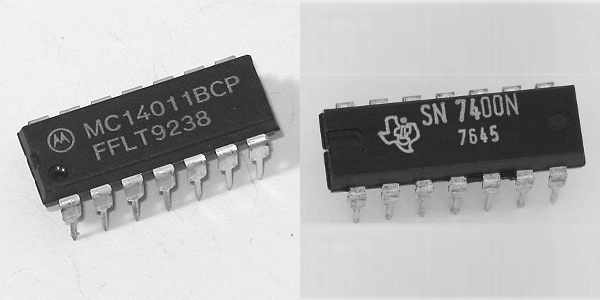
\includegraphics[height=3cm]{transistores.png}
    \caption{Integrados con tecnologías CMOS (izquierda) y TTL 
    (derecha)}\label{fig:transistores}
\end{figure}

Las diferencias entre los transistores de tecnología BJT y los de 
tecnología FET, vienen dadas por la forma en la que cada tipo de 
componente controla el paso de corriente de la terminal colectora a 
la emisora: mediante los campos magnético inducidos en la unión de 
materiales dopados con átomos de diferente capacidad de difusión
de cargas (positivas y negativas), en el caso de los transistores de
unión bipolar; o mediante un aislante que modifica su característica
dieléctrica al aplicársele una tensión. En la Figura 
\ref{fig:transistores} mostramos ejemplos de integrados para ambas 
tecnologías.

A continuación listaremos sus principales diferencias:

\begin{itemize}
    \item {
        Los integrados desarrollados con CMOS son en general más 
        costosos que su contraparte TTL.
    }
    \item {
        Los integrados con tecnología TTL son más robustos contra
        las descargas de estáticas.
    }
    \item {
        La propagación es más rápida en los TTL que en los CMOS. 
        Estas últimas características hacen que los TTL sigan siendo
        utilizados.
    }    
    \item {
        La dimensión de los CMOS es mucho menor que la de los TTL.
    }
    \item {
        Al operar con baja corriente, los CMOS tienen menos consumo 
        que los TTL. Estas últimas características han hecho que los 
        CMOS se transformaran en los más utilizados en la industria.
    }
    \item {
        Además, los niveles de tensión para los integrados con TTL 
        rondan los 5 voltios mientras los márgenes para los CMOS son
        mucho mayores: desde los 3 a los 18 voltios.
    }
    \item {
        La cantidad de salidas que pueden conectarse a un CMOS sin 
        alterar el correcto funcionamiento (puesto que funcionan con
        baja corriente) es cinco veces superior a las que permite un 
        TTL. Sin embargo, la cantidad de entradas posibles son 
        levemente superiores en estos últimos.
    }
    \item {
        Con los TTL encontramos en general implementaciones de puertas
        NAND, mientras que tanto puertas NAND como NOR son comunes en
        integrados con transistores del tipo CMOS.
    }
    \item {
        Si bien no es una regla infalible, los integrados con 
        tecnología TTL suelen indicarse con etiquetas de la serie 
        7XXX, y los de tecnología CMOS con etiquetas del tipo 4XXX.
    }
\end{itemize}

\section{Descripción de la Práctica}

\subsection{Enunciado}

A continuación transcribimos el enunciado original de la práctica.
Del mismo tomamos los puntos teóricos que son descriptos en la 
Introducción. Los ejercicios prácticos son desarrollados en la sección
Diseño y Simulación.

\begin{quotation}

    \begin{center}

        Laboratorio de Microprocesadores - 2020
        
        Taller de Microprocesadores Trabajo Practico  2                

    \end{center}

    \begin{enumerate}

        \item{
            Describir brevemente las características de las entradas 
            analógi-cas del chip. Determine cuantos niveles se pueden 
            detectar en una entrada analógica y cual es la mínima 
            variación que se puede detectar.
            
            Haga uso de una entrada analógica en el entorno de Proteus,
            detecte un nivel de amplitud de una señal analógica 
            conectada a una de las entradas del chip. Puede detectar 
            si es superior o inferior a cierto valor.
            
            Por ejemplo: puede encender un LED cuando el nivel de una 
            señal analógica supere cierto valor.

            Experimente el uso de instrumentos en el entorno de Proteus.

            Los instrumentos en la simulación serán de mucha utilidad 
            para verificar el funcionamiento del diseño y del programa. 
            Encontrará, entre otros, voltímetro, amperímetro, 
            voltímetro, generador de ondas analógicas, osciloscopio, 
            etc.
        }
        \item{
            Describa brevemente qué es la tecnología CMOS, qué es la 
            tecnología TTL y qué las diferencia.
        }
        \item{
            Qué dispostivo/s emplearía para controlar con el 
            microcontrolador el encendido y apagado de un dispositivo 
            que funciona a una corriente considerable o que funciona 
            con corriente alterna. Implemente un circuito en Proteus. 
            (Puede modificar el circuito realizado para el item 3 del 
            TP1, para encender una lámpara o un motor).
        }
        \item{
            Diseñe el circuito de alimentación del chip PIC12F675 
            considerando que tendrá una fuente de alimentación externa 
            de 9V. La fuente externa es una fuente 220 Vac / 9 Vdc.
        } 
    \end{enumerate}
\end{quotation}

\subsection{Plataforma de Desarrollo}

Utilizamos el lenguaje C para programar las aplicaciones. Presentamos
una copia de los mismos como anexos.

Para nuestro desarrollo utilizamos el compilador MPLAB 
XC8\cite{bib:compilador} de la empresa Microchips. El mismo es el 
diseñado específicamente para la línea de microcontroladores de 8 bits
a la que pertenece el PIC12F675.

El diseño y simulación del esquemático correspondiente a cada 
aplicación se realiza con el software Proteus\cite{bib:simulador} de 
la compañía Labcenter Electronics.

\subsection{Instrucciones de Compilación y Ejecución}

Para la compilación del firmware utilizamos la línea de comandos en 
una terminal. Como parámetro a la ejecución del compilador agregamos
el modelo del microcontrolador donde se instala el software. Éste es 
el método recomendado por el desarrollador por sobre el de incluir en 
el código mismo los archivos de encabezado para el preprocesador con 
las configuraciones específicas del modelo. Por ejemplo, para el 
primer ejercicio utilizamos:

\begin{center}\ttfamily 
	xc8 --chip=12f675 ejercicio1.c
\end{center}

El compilador genera un archivo {\ttfamily .hex} que es el que
agregamos a las propieda-des del microcontrolador solicitadas 
por el software Proteus para la simulación del circuito. Allí también 
indicamos tanto la frecuencia del reloj y la palabra que representa 
los bits de configuración que debieran ser impresos en la memoria del
integrado junto con el código ejecutable. 

\section{Diseño y Simulación}

\begin{ejercicios}

    \subsection{Monitoreo de una señal analógica}\label{ej:monitoreo}

    Para este ejercicio utilizamos el circuito que se ilustra en la
    Figura \ref{fig:esquematico1}. Consta de un LED conectado a masa 
    y al pin 5 ó GP2 del microcontrolador más una señal sinusoidal de
    un hertzio con valores de 0 a 5 voltios de pico a pico 
    conectada al pin 0 ó AN0. Para facilitar la simulación con el 
    \textit{software} Proteus, agregamos una punta de prueba sobre la 
    línea que conduce la señal analógica.
    
    Nuestro microcontrolador ya posee los módulos necesarios para 
    realizar toda la aplicación: un módulo comparador de señales 
    analógicas con la capacidad de entregar el resultado como señal 
    digital en el pin GP2 y un módulo generador de un voltaje de 
    referencia.

    % --- Para insertar una imagen escriban de acá
    \begin{figure}[h]\centering
    % La opcion `[h]` es para "here", pero puede cagarse en eso.
    % No usar "la imagen que sigue" sino la referencia.
        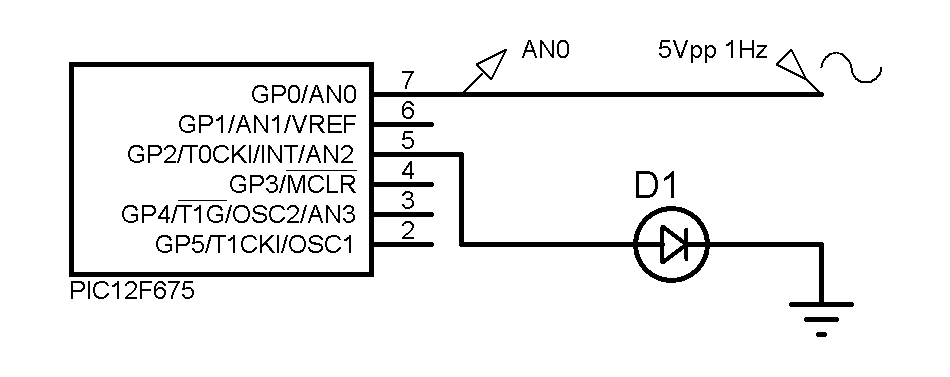
\includegraphics[height=3cm]{esquematico1.png}
        \caption{Esquemático del circuito utilizado en el  
        \ref{ej:monitoreo}}\label{fig:esquematico1}
    \end{figure}
    % --- hasta acá.

    El código fuente para este ejercicio es el que se lista en el 
    \ref{ane:monitoreo}. Vemos que consecuentemente, el mismo sólo
    consiste en la configuración de los módulos que ya posee el 
    microcontrolador (líneas 15 a 19) más un ciclo infinito (línea 21).

    Los registros del microcontrolador se configuran de acuerdo a lo 
    que se indica en su \textit{datasheet}\cite{bid:datasheet}. 
    Brevemente: se enciende el módulo comparador y se le asigna la
    señal proveniente del pin AN0 y la del módulo interno de voltaje 
    de referencia, dirigiendo el resultado al pin GP2 (línea 15); el 
    voltaje de referencia se ajusta a 3.59 voltios para el caso de un
    voltaje de operación de 5 voltios (línea 19); y finalmente se 
    configuran los puertos estableciendo sólo al GP0 ó AN0 como 
    analógico (línea 16) y única entrada (línea 17), siendo los demás
    puertos de salida inicializados en cero (línea 18).

\end{ejercicios}

\section{Conclusiones}
Dummy text que cita a la obra \cite{bib:boylestad}

\noindent\rule{\textwidth}{1pt}
% Linea horizontal sin identacion y del ancho del texto

\begin{thebibliography}{9}
% Comienza la bibliografia
% El "9" indica que el espacio para imprimir "9" es de la mayor referencia

% Para agregar una entrada a la bibliografia repetir de aca
\bibitem{bib:boylestad} 
Boylestad, R. \& Nashelsky, L. (2002). 
\textit{``Electronic devices and circuit theory"}.
Upper Saddle River, N.J: Prentice Hall.
% Hasta aca termina la referencia

\bibitem{bib:compilador}
\textit{``Microchip MPLAB XC8 C Compiler"}
(Versión 2.10; Microchip Technology Inc.: 2019).
Recuperado de https://www.microchip.com/mplab/compilers

\bibitem{bib:simulador}
\textit{``Proteus 8 Professional"} 
(Versión 8.5 Service Pack 0; Labcenter Electronics: 2016).
Recuperado de https://www.labcenter.com/

\bibitem{bid:datasheet}
Microchip (2010).
\textit{``PIC12F629/675 Data Sheet. 8-Pin FLASH-Based 8-Bit CMOS 
Microcontrollers''.}
EE.UU. Recuperado de 
http://ww1.microchip.com/downloads/en/DeviceDoc/41190G.pdf
\end{thebibliography}

\appendix

\section{}\label{ane:monitoreo}
A continuación listamos en extenso el código fuente en lenguaje C
correspondiente al \ref{ej:monitoreo}. La descripción de su 
funcionamiento puede encontrarse en la sección de Diseño y 
Simulación.

\lstinputlisting[language=C,basicstyle=\ttfamily\scriptsize,numbers=left]{../ejercicio1.c}
% `lstinputlisting` inserta el codigo.
% Lo configuro para C, en monospace y tamaño chico, con numeracion a la izquierda.
% Recordar que el archivo tiene una direccion relativa a esta carpeta.
% Los de verdad van a estar en la carpeta padre "../ejercicio1.c"

\newpage
% Incluir salto de pagina de manera manual en cada apendice.
\section{}

\end{document}
